\documentclass[11pt]{article}

\title{Model Checking World Domination}
\author{Jacob Errington \& Kevin Li}
\date{Formal Verification -- COMP 525\\18 April 2017}

\usepackage{tikz}
\usepackage{amsthm,amsmath,amssymb}
\usepackage{csquotes}
\usepackage{ragged2e}
\usepackage[margin=3.0cm]{geometry}
\usepackage{hyperref}
\usetikzlibrary{automata, graphs, arrows}

\theoremstyle{definition}
\newtheorem{defn}{Definition}
\renewcommand{\phi}{\varphi}
\newcommand{\OR}{\mathbin{\big\vert}}
\renewcommand{\P}[2]{\mathcal{P}_{#1}\left(#2\right)}
\newcommand{\until}{\mathbin{\mathtt{U}}}
\newcommand{\X}{\bigcirc}

\newcommand{\abs}[1]{\left\vert{#1}\right\vert}

\begin{document}

\maketitle

\begin{abstract}
    Probabilistic model checking is used to verify properties of a robotic
    swarm performing a certain task.
    %
    Several canonical tasks are studied extensively in the literature,
    such as foraging, flocking, and navigation.
    %
    The problem of robotic swarm task allocation arises when a swarm is
    presented with multiple tasks to complete concurrently: in what proportions
    must a swarm disaggregate and recombine to most efficiently complete all
    tasks?
    %
    Extant literature on robotic swarm task allocation focusses on the
    aforementioned types of tasks.
    %
    In this paper we introduce the notion of distributable probabilistic tasks,
    and propose a probabilistic model checking framework through which optimal
    allocation proportions can be derived.
\end{abstract}

\section{Introduction}
\label{sec:intro}

A robot swarm is a group of robots acting cooperatively to perform a task.
Different types of swarms have been considered in the literature.
Most often, one considers homogeneous swarms, in which the members have
identical capabilities.
Swarm robotics is a notorious field due to issues of \emph{scale}.
It is not necessarily clear what properties a swarm will have when one knows
only the properties of its members.
Contrariwise, knowing only the properties of the swarm in aggregate, it can be
difficult to see what properties the members ought to have.
Hence in the design of robot swarms, there are two major approaches:
%
\begin{enumerate}
    \item
        the \emph{macroscopic} approach focuses on the desired properties of
        the swarm as a whole, and attempts to determine how to build suitable
        member robots; \cite{brambilla12}
        %
    \item
        the \emph{microscopic} approach starts with the design of individual
        robots, and attempts to predict what properties emerge from that
        construction. \cite{brambilla12}
        %
\end{enumerate}

In recent years, robot swarm engineering has evolved from a rather ad hoc
endeavor to a more principled science.
Brambilla, Pinciroli, Birattari, and Dorigo (2012) propose a novel framework
for designing robot swarms: their
methodology is driven by model checking.
As the outcomes of a robot's actions are uncertain, the techniques of
probabilistic model checking are more appropriate.

In applying the principles of model checking to the microscopic approach to
swarm design, one models each member of the swarm as an independent transition
system.
Communication and coordination protocols are modeled as controllers.
The swarm's behaviour can then be studied by examining the properties of the
composed transition system.
As swarms of greater size are modelled in this way, the composition of their
transition systems becomes \emph{factorially} larger.
Due to this state space explosion, microscopic model checking is currently
infeasible for swarms of any appreciable size.

In contrast, the macroscopic approach does not track the internal state of each
robot directly as in the microscopic approach.
Assuming homogeneous robots, the macroscopic approach uses a single
transition system to model the swarm.
This system is obtained by considering the different states a single robot can
be in, and augmenting these states with a count of how many robots of the swarm
are in that state.
The transition rules between states in the augmented system must
govern what \emph{proportion} of robots change state without having access to
the internal details of the particular robots.

In this paper, we follow the macroscopic approach.
By representing the robotic swarm in this way, we can describe and analyze a
much larger system than otherwise possible.
This makes it possible to verify more interesting properties.
%
The scope of this paper does not include the (daunting) challenges involved in
the engineering of a robot swarm, nor do we take into account many practical
considerations such as the reliability of communication between robots or
hardware.
We take an abstract view of a robotic swarm and assume (perhaps recklessly)
that these issues are solved.

This paper is structured as follows.
%
In section \ref{sec:background-motivation} we provide an overview of the
existing literature on probabilistic model checking and on task allocation in
swarm robotics.
We then introduce the problem domain that our framework addresses, along with
the notion of a distributable probabilistic task.
%
In section \ref{sec:model} we describe how our framework is constructed using a
concrete combat example.
%
In section \ref{sec:implementation} we describe the implementation of our
framework, along with the specifications of how our experiments were
implemented.
%
In section \ref{sec:results} we present our experimental results and discuss
their relevance.
%
We conclude in section \ref{sec:conclusion} and consider avenues for future
improvement.

\section{Background and Motivation}
\label{sec:background-motivation}

The results of actions in the real world can be uncertain.
Specifically in a robot swarm, the actions of a particular robot might fail.
Probabilistic models exist to handle this type of situation, and are hence a
tool of choice for modeling robotic swarms.
A transition system for a robot swarm can be augmented with probabilities,
giving rise to a discrete-time Markov chain (DTMC).

Liu, Winfield, and Sa represent a foraging swarm following the macroscopic
approach using a discrete time Markov chain.
Figure \ref{fig:foraging} shows their construction.

\begin{figure}[ht]
    \label{fig:foraging}
    \begin{center}
        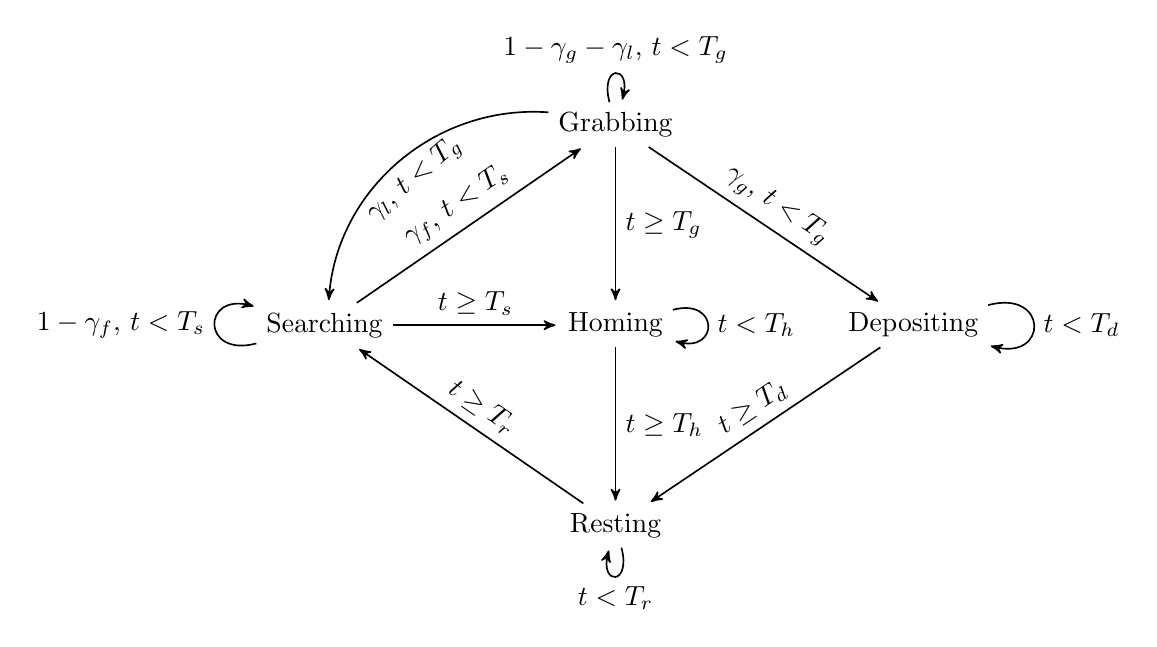
\begin{tikzpicture}[
                ->,
                > =stealth',
                draw=black,
                semithick,
                shorten >=1pt,
            ]
            \matrix[row sep=2cm, column sep=2cm]{
                &
                \node (G) {Grabbing} ; &
                \\
                \node (S) {Searching} ; &
                \node (H) {Homing} ; &
                \node (D) {Depositing} ; \\
                &
                \node (R) {Resting} ; &
                \\
            } ;

            \graph[use existing nodes]{
                S ->[
                    edge label={$1 - \gamma_f$, $t < T_s$},
                    loop left,
                    looseness=4
                ]
                S ->[
                    edge label={$\gamma_f$, $t < T_s$},
                    sloped,
                ]
                G ->[
                    edge label={$1 - \gamma_g - \gamma_l$, $t < T_g$},
                    loop above,
                ]
                G ->[
                    edge label={$\gamma_l$, $t < T_g$},
                    bend right=45,
                    swap,
                    sloped,
                ]
                S
                ;

                G ->[
                    edge label={$\gamma_g$, $t < T_g$},
                    sloped,
                ]
                D ->[
                    edge label={$t < T_d$},
                    loop right,
                    looseness=4,
                ]
                D ->[
                    edge label={$t \geq T_d$},
                    sloped,
                ]
                R ->[
                    edge label={$t < T_r$},
                    loop below,
                ]
                R ->[
                    edge label={$t \geq T_r$},
                    sloped,
                ]
                S ->[
                    edge label={$t \geq T_s$},
                ]
                H ->[
                    edge label={$t < T_h$},
                    loop right,
                    looseness=4,
                ]
                H ->[
                    edge label={$t \geq T_h$},
                ]
                R
                ;

                G ->[
                    edge label={$t \geq T_g$},
                ]
                H
                ;
            } ;
        \end{tikzpicture}
    \end{center}
    \caption{
        Konur, Dixon, and Fisher's foraging swarm representation.
        This model is in fact a probabilistic timed automaton (PTA), but
        dropping all clock guards (of the form $t < T$ or $t \geq T$) yields a
        DTMC.
    }
\end{figure}

The macroscopic representation of this robotic swarm shows that each robot is
responsible for attempting to gather ``food'' in order to increase the overall
energy levels of the entire swarm. The semantics of the states are:
%
\begin{description}
    \item[Searching.] Robot is searching for food.
    \item[Grabbing.] Robot attempts to grab a food item.
    \item[Depositing.] Robot returns home with the food item.
    \item[Homing.] Robot returns home without any food items.
    \item[Resting.] Robot rests for some time.
\end{description}

Then, there are some timeout conditions and probability
distributions over states after a transition is performed.
%
\begin{itemize}
    \item
        $ T_s $ is the maximum amount time a robot can continue searching.
        %
    \item
        $ T_g $ is the maximum amount of time a robot can attempt grabbing.
        %
    \item
        $ T_d = \frac{T_h}{T_r} $ is the average time spent depositing.
        %
    \item
        $ \gamma_f $ is the probability of finding a food item.
        %
    \item
        $ \gamma_g $ is the probability of grabbing a food item.
        %
    \item
        $ \gamma_l $ is the probability of losing sight of a food item.
        %
\end{itemize}

After including timeout conditions in the guards of transitions, the model as
introduced by Konur, Dixon, and Fisher is actually a probabilistic timed
automaton.
However, ignoring the guards on clock values and removing all self-transitions
guarded only by clocks, we can consider this model exactly as a discrete time
Markov chain.
Then, we can see that a robot in the ``Searching'' state can probabilistically
transition into either the ``Grabbing'' state, or continue to search for food
items.

Reward structures can be added to this model to track the total swarm energy
levels.
Each time a food unit is deposited, the overall energy level increases.
Whenever the robots perform actions such as searching for food or returning
home, the overall energy level increases.
This reward structure is used as a proxy for tracking the fuel levels of the
individual robots, which cannot be directly measured due to the nature of the
macroscopic approach.
Nonetheless, properties such as ``With what probability does the overall fuel
level reach zero?'' can be verified and can serve to inform whether the swarm
behaves well in aggregate.

These properties are written in Probabilistic Computation Tree Logic (PCTL)
\cite{pctl}, which extends Computation Tree Logic (CTL) to talk about
probabilities. As in ordinary CTL, probabilistic CTL separates
\emph{state formulas}, denoted with capital Greek letters, and
\emph{path formulas}, denoted with lowercase Greek letters.
%
\begin{align*}
    \Phi &::= \text{true}
        \OR a
        \OR \Phi_1 \land \Phi_2
        \OR \neg \Phi
        \OR \P{\sim \lambda}{\phi} \\
    \phi &::= \X \Phi \OR \Phi_1 \until \Phi_2
\end{align*}
%
where $\sim$ is one of $>$, $<$, $\leq$, or $\geq$ and $\lambda \in [0,1]$ is
a probability.

The satisfaction of $\P{\geq\lambda}{\phi}$ is defined by
``s satisfies $ \mathcal{P}_{\geq\lambda} ( \phi ) $ iff s
satisfies $ \phi $ with probability greater than or equal
to $ \lambda $''.
The $ >, <, \leq $ cases for $ \sim $ follow similarly.
% TODO this explanation of satisfaction feels... *puts on sunglasses*
% unsatisfying.

Hence, the $\exists$ and $\forall$ path operators of ordinary CTL are subsumed
by the probability path operator $\mathcal{P}$: existence of a path satisfying
$\phi$ means there is nonzero probability of $\phi$; requiring that all paths
satisfy $\phi$ means that $\phi$ is satisfied with probability $1$.

% TODO revise below this point.

PCTL properties can be written directly into PRISM, and
given a model that supports the property (i.e. there is
no variable in the property that is not mentioned
in the model) such a property can be verified.
PRISM supports an additional feature: if the $ \lambda $
parameter is not specified in the property, then
instead saying if the property is satisfied or not
satisfied, PRISM will return the probability that
the property is specified. For example, Konur,
Dixon, and Fisher demonstrate the computation of
the probability that ``for an arbitrary number of robots
and food finding probability, the swarm energy is
equal to or greater than the initial energy from
a time point $ t_A $.'' This property can be written
in PCTL as:

\begin{align*}
    P_{=?}((t < t_A) & \vee (E(t) \geq E(0)) \text{ U } t = t_{max} ) \\
    \text{where } & t \text{ is the time variable} \\
                  & t_A \text{ is the designated time point} \\
                  & t_{max} \text{ is the simulation end time} \\
                  & E(t) \text{ is the function returning the energy at time } t
\end{align*}

Thus by constructing a swarm robotics in this way,
PCTL properties can be used to verify probabilistic
properties.

We observe that this foraging task, however, does
not fully leverage the unique capabilities of
a robot swarm. Specifically, the ability
to aggregate and disaggregate. The foraging
task essentially segregates all robots from
each other, and assumes they can act
independently. Furthermore, it does not
consider the possibility for robots to
cooperate with each other to increase
the probability of successfully completing
some task. Because real-world tasks will,
more often than not, be more complex than
the independent foraging task, we define
another slightly more complex type of task
along with real world examples of such tasks.

\begin{defn}
    A \emph{distributable probabilistic task}
    (DPT) is a task (in a discrete time domain)
    where:

    \begin{itemize}
        \item completion of the task by
            the agents working on it
            occurs probabilistically in
            each time step
        \item cooperation of agents working
            on the same task increases the
            completion probability
        \item agents can work on multiple
            tasks concurrently
        \item the tasks may be of different
            difficulty
        \item after completion of a task,
            the agents that were originally
            working on that task may
            redistribute themselves
            among the remaining active tasks.
    \end{itemize}

    We also assume that the swarm robots
    are homogeneous.
\end{defn}

Examples of real-world tasks that roughly
fit this model are:

\begin{itemize}
    \item combat scenarios with multiple enemies.
        Robots are designated targets. Multiple
        robots attacking the same target
        improves the chances of taking down
        a target in any given round of combat.
    \item cryptocurrency mining. A mining pool
        can allocate computational resources to
        try and compute correct hashes to
        obtain a block of a particular
        cryptocurrency.
    \item DDOS attack planning. A botnet's
        output capacity (measured in bits/second)
        can be allocated among different servers
        to try and overload them.
    \item search and rescue. Several collapsed
        buildings can be considered different
        adversaries, where fully exploring
        and identifying rescue targets occurs
        probabilistically due to uncertainty
        in the layout of a collapsed building.
        Cooperative search and rescue efforts improves
        the likelihood of completing search efforts
        in a building.
\end{itemize}

For the remainder of this paper, we primarily
refer to the combat example when talking about
our model.

For DPTs, task allocation becomes an interesting
problem.
Specifically, given $ N $ enemies,
with the ith enemy having some difficulty
rating $d_i$ (measuring how difficult it is
to defeat that enemy), how should we allocate our robots
in order to optimize for some desired effect
(e.g. probability of victory, probability of maximum
survival?)
When considering the method by which we should allocate
robots between enemies, it is important to realize
that battles may conclude at different times, and
thus it is important not only to specify how the
swarm should \emph{initially} be allocated,
but also how a group of robots should reallocate
themselves when a battle is won. We treat this
as an optimization problem and in section
\ref{sec:model}, we construct a model that
will allow us to produce an optimal allocation
policy for enemies.

\section{Model Construction}
\label{sec:model}

Conceptually, we represent a combat scenario in the following way.

We are given $ N $ robots and the set of enemies
$ M \subset \mathbb{N} \times \mathbb{R} $,
where the first element of the tuple is the unique identifier
of the enemy, and the second element is the difficulty level
of the enemy. These $ N $ robots may be distributed
in any way between all $ \abs{M} $ enemies.

We assume that rounds of combat occur concurrently in discrete time,
and that in any given round of combat against a
particular enemy, that enemy may be defeated
with some probability.

Furthermore, if more robots are fighting
the same enemy, then the probability of
defeating that enemy is higher.

Finally, after an enemy is defeated, all of
the robots that were originally fighting
that enemy can redistribute themselves
over the remaining battles.

\begin{figure}
    \caption{Transition system representation battle $ i $}
    \label{tikz:battle}
    \centering
    \begin{tikzpicture}
        \matrix[row sep=3cm,column sep=3cm]{
            \node[draw=black,circle] (s0) {$s_0$} ; &
            \node[draw=black,circle] (s1) {$s_1$} ; &
            \node[draw=black,circle] (s3) {$s_3$} ; &
            \node[draw=black,circle] (s4) {$s_4$} ; \\
            &
            \node[draw=black,circle] (s2) {$s_2$} ; &
            &
            \node[draw=black,circle] (s5) {$s_5$} ; \\
        } ;

        \graph[use existing nodes] {
            s0 ->[edge label={init}] s1 ;
            s1 ->[edge label={attack, $ p_i$},bend left=30] s2 ;
            s1 ->[edge label={attack, $ 1 - p_i $}] s3 ;
            s2 ->[bend left=30] s1;
            s3 -> s4;
            s4 ->[edge label={attack},loop right] s4;
            s4 ->[edge label={done}] s5;
        } ;

    \end{tikzpicture}
    \small
    \justify
    \par
    Each battle is conducted concurrently. So once we
    have observed the set of enemies, we can construct
    a transition system that looks like this for each enemy,
    and then construct the composed transition system.
    %
    In the composed transition systems, all labeled actions
    must be performed synchronously between all
    transition systems. These actions are "attack", "done", and "init".
    %
    Due to our assumption that rounds of combat
    occur in discrete time, and are concurrent,
    all attacks will occur in lockstep, and
    we will assume that redistribution is instantaneous.

    The description of the states follow.

    \begin{itemize}
        \item $ p $ is the probability of defeating the current
            enemy in a round of combat.
        \item $ s_0 $ is the state in which all battles start.
            The "init" action synchronizes across all
            battles, so the initial
            distribution of robots occurs at the same time
            across all battles.
        \item $ s_1 $ is the "ready" state in which
            attacking can occur. When the "attack" action
            occurs, the battle can transition into
            $ s_2 $ with probability $ p_i $, or
            $ s_3 $ with probability $ 1 - p_i $.
        \item $ s_2 $ is the state representing the result
            of a non-victorious attack. Because
            the transition back to $ s_1 $ does not
            have a label, the return to $ s_1 $ is
            performed non-synchronously by different battles.
            This is important later when we incorporate
            our notion of casualties in combat.
        \item $ s_3 $ is the state representing the result
            of a victorious attack. The transition
            leading from $ s_3 $ to $ s_4 $ contains
            the reallocation of all robots in the
            current battle to all remaining battles.
        \item $ s_4 $ is the state representing the
            conclusion of a single battle.
        \item $ s_5 $ is the state representing the
            conclusion of all battles. This state
            can only be entered with the "done" action,
            which is synchronized across all battles.
    \end{itemize}

    We call $ p_i $ the probability of a failed
    attack in battle $ i $. This probability
    is a function of the difficulty level $ d_i $,
    efficiency of robots $ c $, and
    the current number of robots $ n_i $ fighting
    enemy $ i $.
\end{figure}

In figure \ref{tikz:battle} we mention that the probability
of a failed attack $ p_i $ in battle $ i $ is a function of the
difficulty level of enemy $ i $ ($ d_i $),
efficiency of robots ($c$), and
the current number of robots $ n_i $ fighting enemy
$ i $. Any function that produces a probability can be
used, but in our implementation we use the cumulative
distribution function (figure \ref{fig:exp-cdf}) of an exponential
random variable for the probability of a successful attack.
%
Thus, we use $ e^{-\lambda x} $ as the probability
of a failed attack.
%
Intuitively, the probability of failed attack
increases as the difficulty level of enemy increases.
This is reflected as $ x $ is the difficulty level
of the enemy. Then, we would like for efficiency of
robots and the current number of robots to affect
the probability of a failed attack. Again,
intuitively, the probability of a failed attack
decreases both as the number of robots attacking
the enemy ($n_i$) and the efficiency of robots ($c$)
increase. We encode this in the lambda
parameter of the exponential c.d.f., by setting
$ \lambda = \frac{1}{c n_i} $. This probability
then updates whenever the total number of robots
changes during updates, which occur when casualties
are incurred or when a battle ends and its robots
are redistributed.

\begin{figure}
    \caption{Cumulative distribution function of an exponential random variable with parameter $\lambda$}
    \label{fig:exp-cdf}
    \centering
    $$ f(x) = 1 - e^{-\lambda x} $$
\end{figure}

After a battle concludes, the robots that were
in that battle may redistribute over the remaining battles.
We would like for this redistribution policy
to be agnostic in how it decides to reallocate
bots given the remaining battles' difficulty
levels and number of robots fighting at those battles.
Furthermore, we would like for the redistribution
policy to have some free variable(s) that can be
tuned in order to optimize for certain properties.
%
So we define the redistribution policy as a weighted
average of a function of the adjusted difficulty
($\frac{d_i}{c n_i}$ using our previous notation).

In other words, when battle $ i $ has ended,
let $ \mathcal{F} = \{ j \text{ s.t. } j \neq i \wedge \text{ Battle } j \text{ not ended.} \} $.
%
Our goal is to redistribute $ n_i $ bots among
all $ j \in \mathcal{F} $.
%
For all $ j \in \mathcal{F} $, let $ d_j $ be enemy
$j$'s difficulty level, and let $ n_j $ be the number
of robots currently attacking $j$. Enemy j will
receive:

$$ n_i \frac{g(\frac{d_j}{cn_i})}{\displaystyle\sum_{k \in \mathcal{F}}g(\frac{l_k}{cn_k})} $$

where $ g(x) $ is some scaling function that has at least
one free variable in it that can be tuned.

Then, this model along with the redistribution
policy can be encoded in some model checking software
to calculate properties. Grid search or hill-climbing can
then be used to find the optimal parameterization of
the scaling function $ g(x) $.

In our implementation, we use the scaling function
$ g(x) = x^a $, where $ a $ is our free variable.
However, realistically any non-negative function
can be used.

In order to more accurately capture a battle, we include
the notion of casualties: if a battle is not won in a round
of combat, then the robot swarm will suffer
a single casualty with some probability $ p_c $.
This parameter is also a parameter of the model
that must be specified, like the efficiency of the robots.

An example workflow would follow these steps:

\begin{enumerate}
    \item Select the properties whose probabilities
        you would like to maximize
    \item Construct the model by specifying
        the set of enemies, number and efficiency of robots,
        scaling function, and probability of casualty.
    \item Calculate the probabilities of the
        desired properties while iterating over
        values of parameters for the scaling function.
        Stop when a local maximum for the properties is
        reached.
\end{enumerate}

\section{Experiment Implementation}
\label{sec:implementation}

To show that models of distributable probabilistic tasks can be realistically
analyzed on stock hardware, we wish to verify a number of properties across a
range of DPTs.
Each DPT that we analyze is a concrete instance of the general combat model
outlined in the previous section.
To verify the properties of interest, we must implement each DPT in the PRISM
language.
This means choosing how many ``battles'' will be fought by the swarm and
writing one PRISM module per battle.
(In PRISM, a module corresponds to an individual transition system.)
However, the structure of each transition system is essentially the same, so
writing each of these modules by hand is quite tedious.

To alleviate this, we wrote a PRISM code generator.
This software allows us to express, in an embedded domain-specific language, a
PRISM model.
We then wrote a small front-end for the code generator in which one specifies
how many tasks the swarm must complete.
The output is a PRISM model with the boilerplate code of all the necessary
PRISM modules filled in for the analysis of the corresponding DPT setup.

Next, we need to vary parameters such as the probability of a robot dying or
the efficiency of individual robots to see what effect this has the overall
outcome of the battles.
%
At first, one might think of using PRISM's built-in parametric model checking
facilities.
%
In doing so, the practitioner leaves one or more variables in a PRISM model
undefined.
%
These act as parameters which PRISM can then instantiate with concrete values
following a specification.
%
However, PRISM does not make efficient use of multicore machines:
models are checked serially.
This makes model checking across a wide range of parameters prohibitively slow.

Rather than use PRISM's built-in parametric model checking facilities, we
extended the code generator to support the specification of \emph{all} the
relevant properties for DPTs.
%
In particular, our frontend supports specifying the number of robots in the
swarm, the number of enemies and their difficulty ratings, the efficiency
rating of the robots, and the lethality rating of battle.
%
The output is a concrete PRISM model that can be checked directly.
%
Verifying multiple models in parallel can be done easily with GNU Parallel
\cite{parallel}.

Still, verifying a very large number of models using a single multicore machine
would take quite a long time.
For our purposes, we used three Amazon Web Services Elastic Cloud Compute
servers, each with 16 CPU cores and 30GB of main memory.
Engineers interested in the details of this cloud setup are invited to see the
code online\footnotemark.

\footnotetext{\url{https://github.com/tsani/tortoise}}

\section{Experimental Results}
\label{sec:results}

\section{Conclusion}
\label{sec:conclusion}

% Issues: Not enough parameters to allow for all
% kinds of allocations.
% Can't do this optimization in a reasonable amount
% of time/space with more than 4 enemies.
% Improvements: Same enemies -> use counter instead
% of explicit composition.
% 
% PRISM has parametric model checking, which
% would vastly speed up our process if it were
% not the case that our parameters are all
% involved in the updates.

\section{References}

\begin{thebibliography}{99}
    \bibitem{konur12}
        S. Konur, C. Dixon, and M. Fisher.
        Analysing robot swarm behaviour via probabilistic model checking.
        Robotics and Autonomous Systems, 60:199–213,
        2012.
    \bibitem{konur10}
        Savas Konur, Clare Dixon, Michael Fisher.
        Formal verification of probabilistic swarm behaviours,
        Proceedings of the 7th international conference on Swarm intelligence,
        September 08-10, 2010, Brussels, Belgium
    \bibitem{foraging}
        Liu, W., Winfield, A., Sa, J.:
        Modelling Swarm Robotic Systems: A Study in Collective Foraging.
        In: Proc. Towards Autonomous Robotic Systems (TAROS).
        pp. 25–32 (2007)
    \bibitem{pctl}
        Hansson, Hans, and Bengt Jonsson.
        ``A logic for reasoning about time and reliability.''
        Formal aspects of computing 6.5 (1994): 512-535.
    \bibitem{brambilla12}
        Brambilla M., Carlo P., Birattari M., and Dorigo M.
        "Property-driven design for swarm robotics".
        Proceedings of the 11th International Conference on
        Autonomous Agents and Multiagent Systems.
        AAMAS 2012.
    \bibitem{parallel}
        Tange O.
        ``GNU Parallel - The Command-Line Power Tool'',
        ;login: The USENIX Magazine,
        volume 36, number 1, February 2011,
        Frederiksberg, Denmark,
        pp. 42-47,
        \url{http://www.gnu.org/s/parallel}
\end{thebibliography}

\end{document}
